% https://medium.com/@knownsec404team/analysis-of-the-xz-utils-backdoor-code-d2d5316ac43f
% https://www.openwall.com/lists/oss-security/2024/03/29/4
% https://research.swtch.com/xz-script
% https://www.reddit.com/r/programming/comments/1bv8k7f/the_role_of_ifunc_in_the_xz_backdoor/
% https://github.com/openssl/openssl/blob/master/crypto/rsa/rsa_crpt.c#L51
% https://gitlab.com/cy4n/talk-backdoorxz-pub/-/raw/main/xz_gpn.pdf
% https://gist.github.com/thesamesam/223949d5a074ebc3dce9ee78baad9e27
\section{Backdoor Exploration}

According to \cite{wysopal2007static}, a backdoor refers to a hidden method of
gaining entry to a system bypassing security measures, such as biometric or
password based authentication. They can be implemented in cryptographic
algorithms, on the hardware level or in an application. Backdoors can be used
to remotely access systems and are often hidden inside commonly used
non-malicious software.

\subsection{Implementation}

\texttt{CVE-2024-3094} was assigned to the \texttt{libzlma} backdoor with the
highest possible CVSS Score: $10.0$. This assessement was made due to the
severness of the included remote code execution \cite{redhat2024cve}. The
sophistication of this backdoor suggests a highly proficient attacker known by
several confirmed aliases, such as \textit{Jia Tan} (\texttt{JiaT75}),
\textit{Jigar Kumar}, \texttt{krygorin4545}, \texttt{misoeater91} and
\textit{Hans Jansen} \cite{arstechnica2024xzutils}.

\subsection{Social Engineering \& Pressure on OSS Maintainer}

The process of injecting oneself into the group of maintainers of a open source
software project is a complicated and tedious one. OSS-projects are often led
by a close group of individuals, which often proved themselves by contributing
constructive additions over a long period of time.

A threat actor, whether state-sponsored or a group of individuals, most often
do not take this approach to tampering with software for the purpose of
implementing a backdoor. However this particular backdoor was implemented with
said path over the course of three years.

Specifically the threat actor abused the mental state of the lead maintainer by
applying pressure on them via sock puppet accounts\footnote{false online
identity created and used specifically for deceptive purposes} and depicting
the project changes made by the lead maintainer as slow and not begin up to
date enough. Using said pressure in combination with the maintainers mental
health issues enabled the threat actor to gain the trust and therefore the
co-maintainer position \cite{arstechnica2024xzutils}. 

This position allowed the threat actor to make changes to the build-pipeline,
test files and to sign-off and release versions of the software itself to the
public.

\subsection{Build Pipeline Manipulation}
\label{sec:build_pipeline}

As introduced before, the attacker uses this privileged position in the
maintainer group to make changes to the test files by introducing a file
called \texttt{build-to-host.m4}\footnote{unix macro processor used in
\texttt{autoconf} \cite{gnu2021m4}} \footnote{produces scripts to configure
software \cite{gnu2020autoconf}}. This file is included in the package
release, but not in the version controlled repository. Furthermore the
threat actor embeds obfuscated and encrypted stages of the backdoor in two
test files called \texttt{bad-3-corrupt\_lzma2.xz} and
\texttt{good-large\_compressed.lzma}.

\begin{figure}[H]
    \centering
    \begin{tabular}{c c c}
        Byte & ASCII & Substitution \\
        \hline
        \texttt{0x09} & \texttt{"\textbackslash t"} & \texttt{0x20}\\
        \texttt{0x20} & \texttt{" "} & \texttt{0x09} \\
        \texttt{0x2d} & \texttt{"-"} & \texttt{0x5f} \\
        \texttt{0x5f} & \texttt{"\_"} & \texttt{0x2d} \\
    \end{tabular}
    \label{table:replacements}
    \caption{Substitution table according to \cite{arstechnica2024xzutils}}
\end{figure}

The aforementioned macro is executed during the build process and
substitutes characters in the \texttt{bad-3-corrupt\_lzma2.xz} file, as
shown in \autoref{table:replacements}. Upon having performed the
substitution, the \texttt{.xz} file is decoded and ready for the first stage
of the backdoor. 

\subsection{IFUNC \& CPU Features}

\texttt{IFUNC}, short for GNU indirect function is a mechanism for resolving a
function call to an implementation. This is done by invoking the resolver of
said function upon the functions initial invocation. Marking a function with
\texttt{ifunc} allows for the symbol value resolution at load time, for
instance of a shared object. This process is made possible by using the
\texttt{STT\_GNU\_IFUNC} symbol type ELF standard extension. This functionality
is used to replace a generic function implementation with a platform and
architecture specific and often optimized implementation. However there are
some requirements and safe guards for using \texttt{ifunc}: firstly the
attributed function can not be marked as \texttt{weak}\footnote{declare symbol
as weak and not global, allows for overriding}, the resolver and the indirect
function have to be defined in the same translation unit and \texttt{glibc} is
required \cite{gnu2012gcc}.

\begin{listing}[H]
    \begin{minted}[breaklines]{c}
#include <stdio.h>
#include <stdlib.h>

void generic_function_linux() { puts("linux"); }

void generic_function_windows() { puts("windows"); }
    \end{minted}
    \label{code:example_ifunc_implementations}
    \caption{\texttt{ifunc} platform specific function}
\end{listing}

Would one require a function to be executed on specific runtime conditions,
such as conditionally use a faster implementation for the current architecture,
one could make use of the \texttt{ifunc} attribute as follows. \texttt{ifunc}
requires an implementation, as shown in
\autoref{code:example_ifunc_implementations}. And a resolver, see
\autoref{code:example_ifunc_resolver}. The compiler requires the function
implementation signatures to match the function marked with the attribute.

\begin{listing}[H]
    \begin{minted}[breaklines]{c}
void (*select_generic_function())() {
#ifdef __linux__
  return generic_function_linux;
#elif _WIN32
  return generic_function_windows;
#else
  return NULL;
#endif
}
    \end{minted}
    \label{code:example_ifunc_resolver}
    \caption{\texttt{ifunc} function resolver}
\end{listing}


As introduced before, the usage of \texttt{ifunc} introduces symbols with the
\texttt{STT\_GNU\_IFUNC} in the ELF symbol table in the resulting binary. These
entries point to their respective resolver functions.

\begin{listing}[H]
    \begin{minted}[breaklines]{c}
void generic_function() __attribute__(
(ifunc("select_generic_function")));

int main() {
  generic_function();
  return EXIT_SUCCESS;
}
    \end{minted}
    \label{code:example_ifunc_attribute}
    \caption{\texttt{ifunc} function stub and function usage}
\end{listing}

The dynamic linker resolves the symbols at load time by calling the resolver
function and patching the symbol with the correct address. 

\begin{listing}[H]
    \begin{minted}[breaklines]{c}
void generic_function_malicious() {
    puts("linux");
    system("whoami"); 
}
    \end{minted}
    \label{code:example_ifunc_backdoor}
    \caption{\texttt{ifunc} malicious function}
\end{listing}

While there are a number of legitimate uses of this feature the threat actor
used \texttt{ifunc} to overwrite \texttt{RSA\_public\_decrypt()}\footnote{used
for implementing RSA decryption \cite{openssl2022rsacrpt}} of the
\texttt{OpenSSL} project with a call to \texttt{system()}\footnote{run sub
programs \cite{gnu2023system}}, executing injected shell code after successful
authentication, thus effectively having introduced a remote code execution
vulnerability. 
Considering the example laid out in \autoref{code:example_ifunc_resolver},
\autoref{code:example_ifunc_implementations} and
\autoref{code:example_ifunc_attribute}, one can observe a severely simplified
implementation of said backdoor in
\autoref{code:example_ifunc_implementations}. The simplified backdoor, see
\autoref{code:example_ifunc_backdoor} and
\autoref{code:example_ifunc_backdoor_resolver}, mimics the way \texttt{liblzma}
was included in the resulting binary by inserting the call to the malicious
implementation thereby replacing the resolver logic and enabling the execution
of shell code. While this allows for a reduced overview over the inner workings
of the backdoor, the complexity of said backdoor is significantly larger than
shown here.

\begin{listing}[H]
    \begin{minted}[breaklines]{c}
void (*select_generic_function())() 
{
  return generic_function_malicious;
#ifdef __linux__
  return generic_function_linux;
#elif _WIN32
  return generic_function_windows;
#else
  return NULL;
#endif
}
    \end{minted}
    \label{code:example_ifunc_backdoor_resolver}
    \caption{manipulated \texttt{ifunc} function resolver definition}
\end{listing}

As introduced before, the first stage of the backdoor is to manipulate the
build pipeline to produce a malicious bash file for producing a shared object
containing the backdoor. Specifically this includes the changes from
\autoref{sec:build_pipeline} and an other file introduced in
\autoref{sec:build_pipeline}, \texttt{good-large\_compressed.lzma}.

Firstly, said file is decompressed via the \texttt{xz} command line
application. The resulting blob is then stripped of junk data with the
\texttt{head} unix tool, while a portion is discarded and subsequently
deciphered using a custom substitution cipher. Once the data is deciphered, the
\texttt{xz} suite is used to decompress the resulting blob. 

\begin{figure}[H]
    \centering

    \tikzstyle{startstop} = [rectangle, rounded corners, minimum width=3cm, minimum height=1cm,text centered, draw=black, fill=red!30]
    \tikzstyle{process} = [rectangle, minimum width=3cm, minimum height=1cm, text centered, draw=black, fill=orange!30]
    \tikzstyle{arrow} = [thick,->,>=stealth]
    \begin{tikzpicture}[node distance=2cm]
        \node (start) [startstop] {.lzma file};
        \node (xz) [process, below of=start] {xz};
        \node (head) [process, below of=xz] {head};
        \node (cipher) [process, below of=head] {cipher};
        \node (end) [startstop, left=1cm of start] {bash file};

        \draw [arrow] (start) -- node[anchor=west] {decompress} (xz);
        \draw [arrow] (xz) -- node[anchor=west] {strip junk} (head);
        \draw [arrow] (head) -- node[anchor=west] {decipher} (cipher);
        \draw [arrow] (cipher.east) -- ++(1,0) |- node[anchor=west] {} (xz);
        \draw [arrow] (xz.west) -- ++(-1,0) -- node[anchor=east] {} (end.south);
    \end{tikzpicture}
    \label{chart:dependecies}
    \caption{Stage 1: backdoor prep}
\end{figure}

The resulting text is used as the starting point for the second stage of the
backdoor, specifically this stage encloses the extraction of the backdoor.


\subsection{Indirect Dependence on libzlma}
\label{sec:dependence}

\begin{figure}[H]
    \centering

    \tikzstyle{startstop} = [rectangle, rounded corners, minimum width=3cm, minimum height=1cm,text centered, draw=black, fill=red!30]
    \tikzstyle{process} = [rectangle, minimum width=3cm, minimum height=1cm, text centered, draw=black, fill=orange!30]
    \tikzstyle{arrow} = [thick,->,>=stealth]
    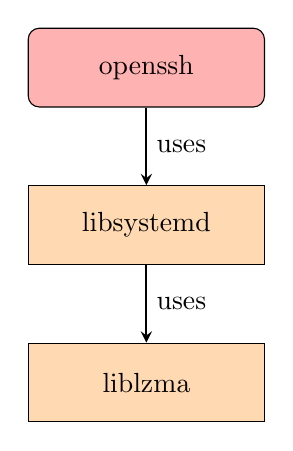
\begin{tikzpicture}[node distance=2cm]
        \node (start) [startstop] {openssh};
        \node (libsystemd) [process, below of=start] {libsystemd};
        \node (liblzma) [process, below of=libsystemd] {liblzma};

        \draw [arrow] (start) -- node[anchor=west] {uses} (libsystemd);
        \draw [arrow] (libsystemd) -- node[anchor=west] {uses} (liblzma);
    \end{tikzpicture}
    \label{chart:dependecies}
    \caption{\texttt{openssh} dependency graph}
\end{figure}

\texttt{openssh} does not directly depend on the \texttt{libzlma} library,
however a number of systems patch \texttt{openssh} to integrate
\texttt{libsystemd} for the purpose of supporting \texttt{libsystemd}
notifications\footnote{used to notify the \texttt{systemd} about status
changes}. This indirect dependencies is dangerously obscure due to the
indirection. The indirection is not only obscure, but also enables the loading
of shared objects of every node in the cascading dependence chain. 

In this chain of shared objects, the threat actor decided to attach the
\texttt{liblzma} backdoor. Specifically the backdoor is active once
\texttt{openssh} loads the \texttt{libsystemd} dependency. Once this dependency
is attempted to be loaded, it starts to load its own dependencies, here the
backdoored \texttt{liblzma}. In this linking stage the before explained
hijacking of the \texttt{RSA\_public\_decrypt()} function is performed.

The result of this process is a remote code execution in said function.

\subsection{Prerequisites for the Backdoor}

\begin{itemize}
    \item built with \texttt{GCC} and \texttt{glibc}
    \item shared object is opened on \texttt{x86-64}
    \item built by \texttt{dpkg} or \texttt{rpm}
\end{itemize}

